\documentclass[tikz,border=2pt]{standalone}
\usepackage{amsmath}
\usepackage{pgfplots}
\pgfplotsset{compat=1.18}
\usetikzlibrary{arrows.meta}
\begin{document}
% x'' + x = 0 started at the same position x(0) = 1 with two velocities:
% x'(0) = 0 gives x(t) = cos t, x'(0) = 1 gives x(t) = cos t + sin t. Position alone does not fix the solution.
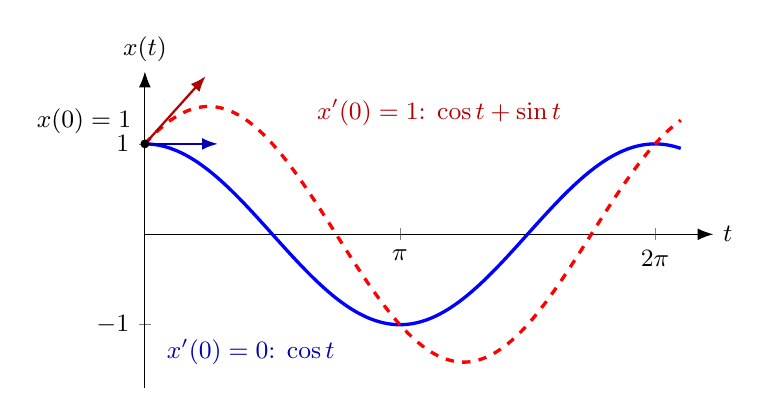
\begin{tikzpicture}[font=\small, >={Latex[length=2mm]}]
  \begin{axis}[width=8.8cm, height=5.6cm, axis lines=middle, axis line style={->},
      xmin=0, xmax=7.0, ymin=-1.7, ymax=1.8, xtick={3.14159,6.28319}, xticklabels={$\pi$,$2\pi$},
      ytick={-1,1}, xlabel={$t$}, ylabel={$x(t)$},
      xlabel style={anchor=west}, ylabel style={anchor=south},
      tick label style={font=\small}, domain=0:6.6, samples=150, clip=false]
    \addplot[blue, very thick] {cos(deg(x))};
    \addplot[red, very thick, dashed] {cos(deg(x))+sin(deg(x))};
    % tangent directions at t = 0
    \draw[blue!70!black, thick, ->] (axis cs:0,1) -- (axis cs:0.9,1);
    \draw[red!70!black, thick, ->] (axis cs:0,1) -- (axis cs:0.75,1.75);
    \fill (axis cs:0,1) circle (1.6pt);
    \node[anchor=east] at (axis cs:-0.05,1.25) {$x(0)=1$};
    \node[blue!70!black, anchor=west] at (axis cs:0.15,-1.3) {$x'(0)=0$: $\cos t$};
    \node[red!70!black, anchor=west] at (axis cs:2.0,1.35) {$x'(0)=1$: $\cos t+\sin t$};
  \end{axis}
\end{tikzpicture}
\end{document}
